\chapter{Implementacja}
Rozdzia� ten po�wi�cono aby om�wi� spos�b implementacji prototypu aplikacji przy pomocy wymienionych rozdzia� wy�ej technologii.

\section{Baza danych}

Baz� danych stworzono stosuj�c podej�cie Code-First, czyli najpierw zosta�y utworzone obiekty w kodzie reprezentuj�ce poszczeg�lne tabele, a nast�pnie zosta�y one zmapowane przy u�yciu rozszerzenia Entity Framework Core na SQL-ow� baz� danych. Podej�cie takie pozwala na szybkie i wygodne wprowadzanie zmian dzi�ki migracjom. Schemat tego podej�cia przedstawiono na rys.~\ref{fig:schematcodefirst}

\begin{figure}[htp]
	\centering
	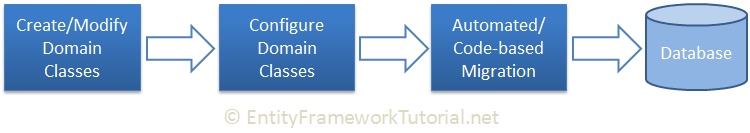
\includegraphics[width=0.7\linewidth]{rys05/dev-workflow.png}
	\caption{Schemat tworzenia bazy danych w podej�ciu Code-First, \cite{CodeFirst}}
	\label{fig:schematcodefirst}
\end{figure}

Schemat zaprojektowanej bazy danych na potrzeby aplikacji przedstawiono na rys.~\ref{fig:schematcodefirst}.
Z powodu du�ej ilo�ci tabel i relacji w schemacie na rys.~\ref{fig:schematcodefirst} nie znalaz�a si� tabela Player.
Tabel� t� wraz z jej relacjami przedstawia rys.~\ref{fig:playerdatabaseschema}.


\begin{figure}[htp]
	\centering
	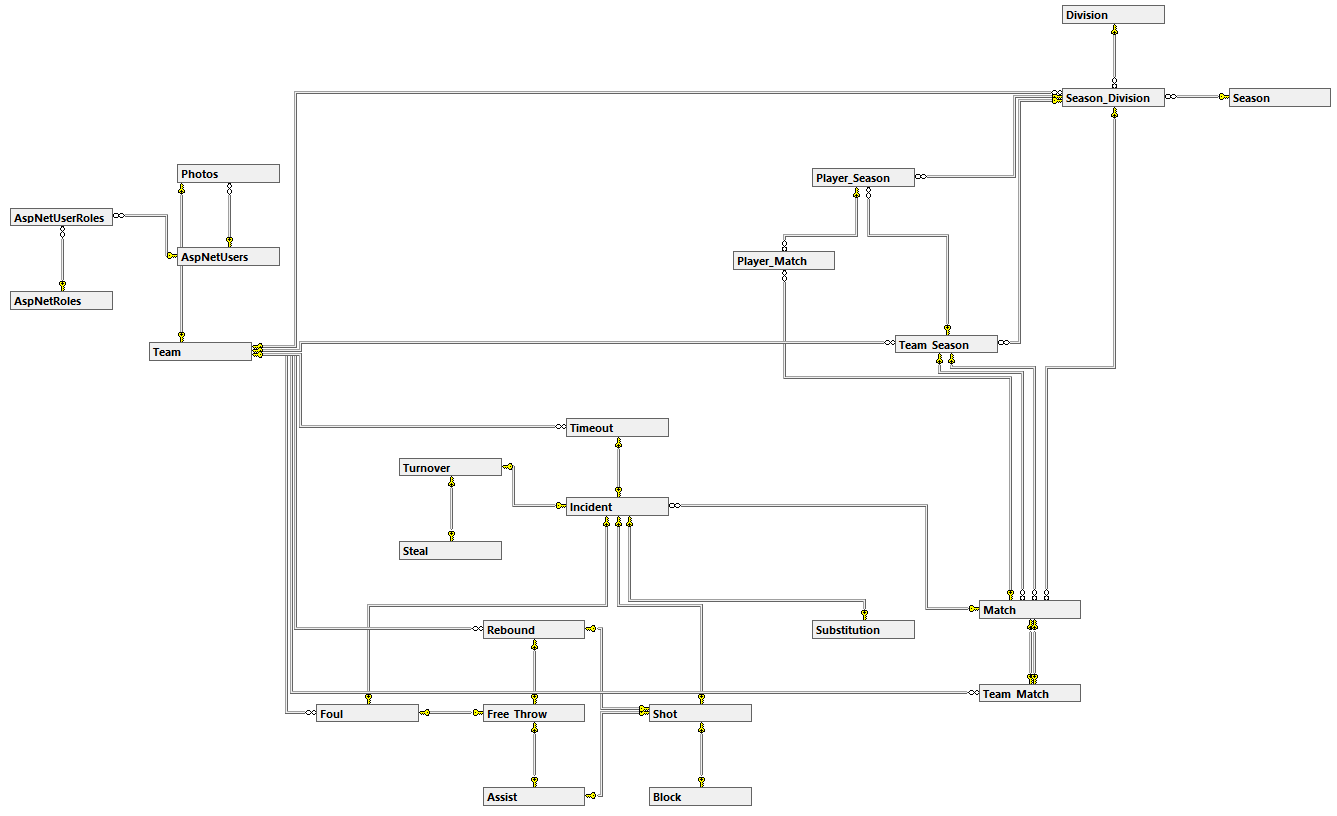
\includegraphics[angle=90, width=0.8\linewidth]{rys05/databaseschema.png}
	\caption{Schemat bazy danych wraz z relacjami (bez tabeli Player)}
	\label{fig:databaseschema}
\end{figure}


\begin{figure}[htp]
	\centering
	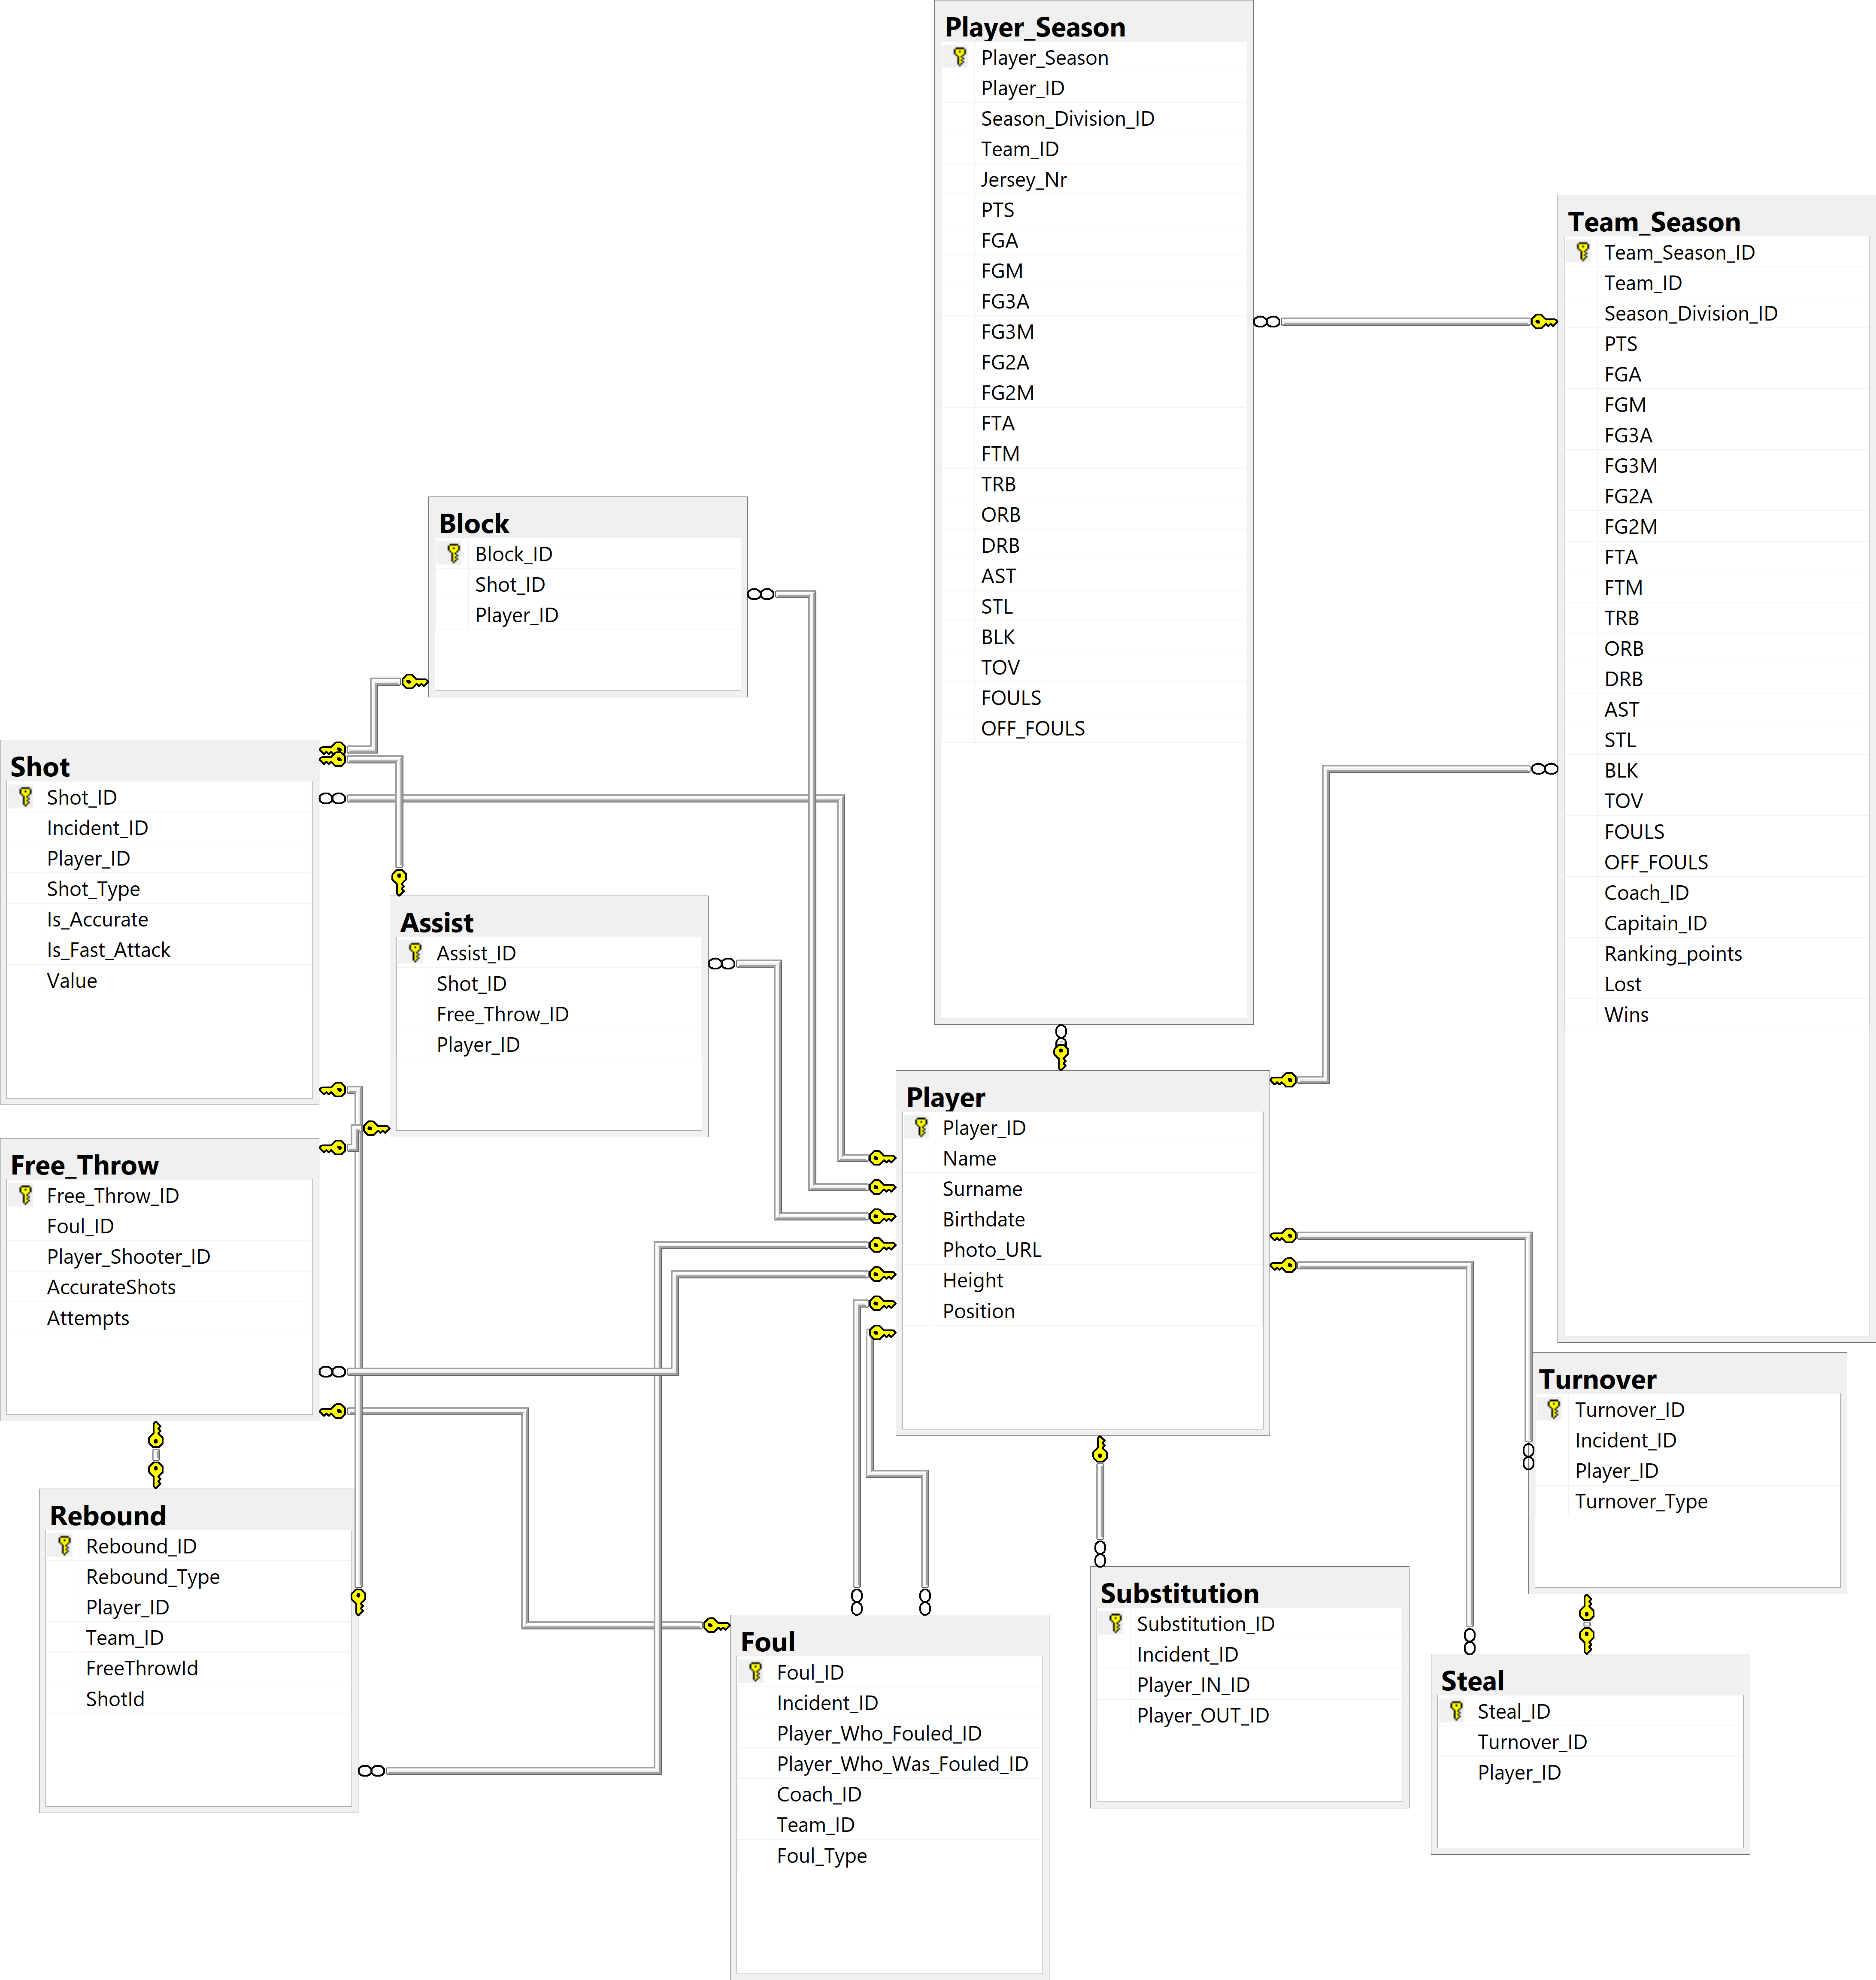
\includegraphics[width=1\linewidth]{rys05/playerdatabaseschema.png}
	\caption{Tabla Player wraz z tabelami relacyjnymi}
	\label{fig:playerdatabaseschema}
\end{figure}






